
\section{B2}
\subsection{B2.1}
\(A)
\R_{1,2} \subseteq S_1 \times S_2 = \{(S_0,S^'_0), (S_1,S^'_1),(S_2,S^'_1),(S_3,S^'_2),(S_4,S^'_3),(S_5,S^'_3),(S_1,S^'_2),(S_0,S^'_3),(S_2,S^'_2),(S_3,S^'_1),(S_4,S^'_0),(S_5,S^'_0),(S^'_0,S_0),(S^'_0,S_4),(S^'_0,S_5),(S^'_3,S_0),(S^'_3,S_4),(S^'_3,S_5),(S^'_1,S_1),(S^'_1,S_2),(S^'_1,S_3),(S^'_2,S_1),(S^'_2,S_2),(S^'_2,S_3)\}
\(B)
\Property (1)
\(S_1,S_2) \in R \rightarrow L_1(S_1) = L_2(S_2)
\newline
\L(S_0)=L(S^'_0)=\{(\phi_1)\}
\L(S_1)=L(S^'_1)=\{(\phi_2)\}
\L(S_2)=L(S^'_1)=\{(\phi_2)\}
\L(S_3)=L(S^'_2)=\{(\phi_2)\}
\L(S_4)=L(S^'_3)=\{(\phi_1)\}
\L(S_5)=L(S^'_3)=\{(\phi_1)\}
\States have same labelling function.
\Property(2)
\forall (S_1, S_2) \in R:
\forall s^'1 \in Post(S_1) \exists S^'2 \in Post(S_2) s.t. (S^'1, S'2) \in R
\newline
\for (S_0, S^'_0)
\S^'_1 \in Post(S_0)=\{(S_1),(S_2),(S_3)\}
\S^'_2 \in Post(S^'_0)=\{(S^'_1),(S^'_2)\}
\(S^'_1, S^_2) \in \{(S_1,S^'_1), (S_2,S^'_2),(S_3,S^'_2)\} \subseteq R.
the same condition for (S_1,S^'_1), (S_2,S^'_1), (S_3,S^'_2), (S_4,S^'_3), (S_5,S^'_3)
\newline
\Property (3)
\forall (S_1, S_2) \in R:
\forall s^'2 \in Post(S_2) \exists S^'1 \in Post(S_1) s.t. (S^'1, S'2) \in R
\newline
\for (S_0, S^'_0)
\S^'_2 \in Post(S^'_0)=\{(S^'_1),(S^'_2)\}
\S^'_1 \in Post(S_0)=\{(S_1),(S_2),(S_3)\}
\(S^'_1, S^_2) \in \{(S_1,S^'_1), (S_2,S^'_2),(S_3,S^'_2)\} \subseteq R.
the same condition for (S_1,S^'_1), (S_2,S^'_1), (S_3,S^'_2), (S_4,S^'_3), (S_5,S^'_3)
\newline
\Property(I) \forall initial states S_1 of T 1 there is an initial state S_2 of T 2 with (S_1, S_2) \in R, and vice versa.
\newline
\as above proved that all properties are verified, this imply T1 and T2 are bisimulation relation. Since we have mapped all the states in M1 is related to a state in M2, so they are maximal.
\newline
\(C)
\R_{1,1} \subseteq S_1 \times S_1 = \{(s_0,s^'_0),(s_0, s^'_4),(s_0, s^'_5),(s_4,s^'_0),(s_4,s^'_4),(s_4,s^'_5),(s_5,s^'_0),(s5,s^'_4),(s_5,s^'_5),(s_1,s^'_1),(s_1,s^'_2),(s_1,s_^'_3),(s_2,s^'1),(s_2,s^'_2),(s_2,s^'_3),(s_3,s^'_1),(s_3,s^'_2),(s_3,s^'_3),(s^'_0,s_0),(s^'_4,s_0),(s^'_5,s_0),(s^'_0,s_4),(s^'_4,s_4),(s^'_5,s_4),(s^'_0,s_5),(s^'_4,s_5),(s^'_5,s_5),(s^'1,s_1),(s^'_2,s_1),(s^'_3,s_1),(s^'_1,s_2),(s^'_2,s_2),(s^'_3,s_2),(s^'1,s_3),(s^'_2,s_3),(s^'_3,s_3)\}
\newline
\(D)
\newline
\R_{1,1} is matces the verified properties,which is same as proved at above the question C.

\(E)
\newline
\begin{center}
Bisimulation quotient M_1/\sim of M_1.
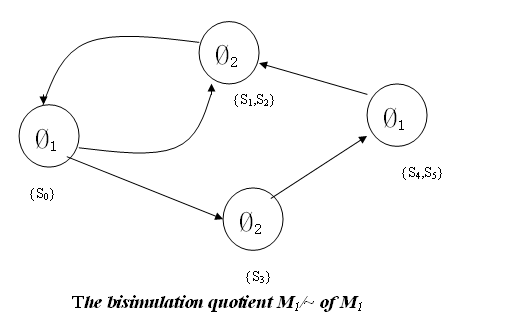
\includegraphics{B2.png}
\end{center}
\newline
\(F)
\Yes, this is bisimilar to M_2. and the largest bisimulation relation between them are:(S_0,S^'_0),(S_0,S^'_3),(S_1,S^'_1),(S_1,S^'_2),(S^_0,S^0),(S^'_3,S_0),(S^'_1,S_1),(S^'_2,S_1)
\begin{center}
\includegraphics{B21F.png}
\end{center}

\subsection{B2.2}

First, the formula is converted into existential normal form:

$\neg (EX \Phi_1) \wedge (\neg (EG \neg \Phi_2))$

The abstract syntax tree consists purely of state formula,
with the path operators included with their enclosing path quantifier:

\begin{figure}[!htb]
\centering
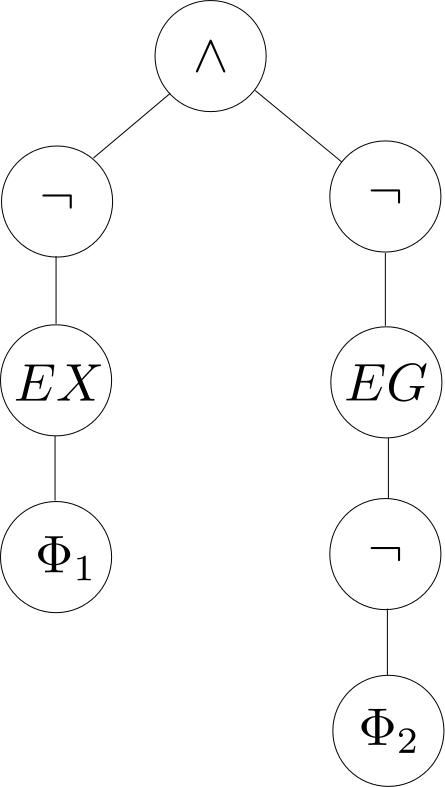
\includegraphics[scale=.4]{abstract_syntax_tree.png}
\caption{Abstract syntax tree}
\label{fig:ast}
\end{figure}

The sub-terms are defined from the atoms up:

$\Phi_1: Sat(\Phi_1)$

$EX \Phi_1: \{s \in S | Succ(s) \cap Sat(\Phi_1) \neq \emptyset\}$

$\neg (EX \Phi_1): S \setminus \{s \in S | Succ(s) \cap Sat(\Phi_1) \neq \emptyset\}$

$\Phi_2: Sat(\Phi_2)$

$\neg \Phi_2: S \setminus Sat(\Phi_2)$

$EG \neg \Phi_2: T, \text{    where } \{s \in S \setminus Sat(\Phi_2) | Succ(s) \cap T \neq \emptyset \} \supseteq T, \text{greatest } T$

$\neg (EG \neg \Phi_2): S \setminus Sat(EG \neg \Phi_2)$

$\neg (EX \Phi_1) \wedge (\neg (EG \neg \Phi_2)): Sat(\neg (EX \Phi_1)) \cap Sat(\neg (EG \neg \Phi_2))$

A sub-term whose set of states is defined recursively is the sub-term $EG \neg \Phi_2$.
The recursion equation is $\{s \in S \setminus Sat(\Phi_2) | Succ(s) \cap T \neq \emptyset \} \supseteq T$.
This equation has many solutions.
Replacing the subset operator with equal, the recursion equation can be seen as a function $f$ of $T$.
The only solutions are then fixed-points of $f$.
A fixed-point for $f$ is a value $x_0$ that makes the following equation true: $x_0 = f(x_0)$,
namely, applying the function to the value gives the value itself, "fixed" in some sense.
It can be shown that the solutions have a unique least solution and a unique greatest solution,
or since the solutions is the same as the fixed-points for the function, a least fixed-point and a greatest fixed-point.
The least fixed-point is the empty set.
The greatest fixed-point is more interesting, and is exactly equal to $EG \neg \Phi_2$.
If the equation had not been an existential-always, but an existential-until or
an existential-eventually, the interesting fixed point would be the least fixed point.

The solution to the transition system $M_1$ can be calculated recursively,
using the sets found for each sub-term:

$\Phi_1: Sat(\Phi_1): \{s_0, s_4, s_5\}$

$EX \Phi_1: \{s \in S | Succ(s) \cap Sat(\Phi_1) \neq \emptyset\}: \{s_1, s_2, s_3\}$

$\neg (EX \Phi_1): S \setminus Sat(EX \Phi_1): \{s_0, s_4, s_5\}$

$\Phi_2: Sat(\Phi_2): \{s_1, s_2, s_3\}$

$EG \neg \Phi_2: \neg \Phi_2: S \setminus Sat(\Phi_2): \{s_0, s_4, s_5\}$

$EG \neg \Phi_2: T, \text{    where } \{s \in Sat(\neg \Phi_2) | Succ(s) \cap T \neq \emptyset \} \supseteq T, \text{greatest } T: \{\}$

$\neg (EG \neg \Phi_2): S \setminus Sat(EG \neg \Phi_2): \{s_0, s_1, s_2, s_3, s_4, s_5\}$

$\neg (EX \Phi_1) \wedge (\neg (EG \neg \Phi_2)): Sat(\neg (EX \Phi_1)) \cap Sat(\neg (EG \neg \Phi_2)): \{s_0, s_4, s_5\}$

